\documentclass[12pt]{article}
\usepackage[a4paper]{geometry}
%\userpackage[top=1 in, bottom=1.25 in, left=1.1 in, rigth=1.1 in] {geometry}
%\usepackage[paperwidth=17cm, paperheight=22.5cm, bottom=2.5cm, right=2.5cm]{geometry}
\usepackage[utf8]{inputenc}
%\usepackage[a4paper, top=2.5cm, bottom=2.5cm, left=2.2cm, right=2.2cm]
%{geometry}
%\usepackage[myheadings]{fullpage}
\usepackage{fancyhdr}
\usepackage{lastpage}
%\usepackage{float}
\usepackage{graphicx, wrapfig, subcaption, setspace, booktabs}
\usepackage{graphicx}
\usepackage[T1]{fontenc}
\usepackage[font=small, labelfont=bf]{caption}
%\usepackage{fourier}
\usepackage[protrusion=true, expansion=true]{microtype}
\usepackage[english]{babel}
\usepackage{sectsty}
\usepackage{url, lipsum}
\usepackage[T1]{fontenc}
\usepackage{icomma}
\usepackage{siunitx}
\usepackage{ragged2e}
\usepackage{amsmath}
\usepackage{comment}
\usepackage{enumerate}
%\usepackage{changepage}
\usepackage{anysize}




\newcommand{\HRule}[1]{\rule{\linewidth}{#1}}
\onehalfspacing
\setcounter{tocdepth}{5}
\setcounter{secnumdepth}{5}

%-------------------------------------------------------------------------------
% HEADER & FOOTER
%-------------------------------------------------------------------------------


\begin{comment}
-Udledninger
$$
\begin{aligned}
\end{aligned}
$$

-Opgavetekst
\begin{figure}[H]
\includegraphics[width=0.5\textwidth]{"path"}
\end{figure} 


-Opgave billede med tekst
\begin{figure}[H]
\caption{"Billedtekst"}
\includegraphics[width=0.5\textwidth]{"path"}
\end{figure} 

-Værdier
$\\
$


\end{comment}
\begin{document}

\begin{titlepage}

\title{ \normalsize 
		%\begin{figure}
        \begin{center}
        
\includegraphics[height=6cm]{Logo.jpg}
        \end{center}
       % \end{figure}
        \LARGE \textsc{\textbf{Universidad De Sonora}} \\ \bigskip
		\Large División de Ciencias Exactas y Naturales \\
        Licenciatura En Física \\ \bigskip
        \bigskip
        Física Computacional I
		\\ [0.1cm]  
		\HRule{2pt} \\
		\Large \textbf{{Actividad 1}} \\
        \textit{\textbf{"Climatología de Guamúchil, Salvador Alvarado"}}
		\HRule{2pt} \\
		\normalsize \vspace*{0.001\baselineskip}}
        
\date{\bigskip \Large  \hspace*{\fill} Hermosillo, Sonora a enero 15 de 2021}

        
\author{
		\Large\textbf{ Ismael Espinoza Arias} \\ \bigskip
        \\ \bigskip
       \Large Profesor Carlos Lizárraga Celaya}
       \end{titlepage}
       \maketitle
       

\newpage
\pagestyle{plain}
\section{Introducción}
 En esta actividad veremos el nombre y número de la estación, coordenadas de Latitud, Longitud y altura sobre el nivel del mar y rango de años de datos disponibles de la ciudad de Guamúchil, ubicada en el municipio de Salvador Alvarado en el estado de Sinaloa. También contaremos con algunos recursos estadísticos, como lo son gráficas de lluvias/mes, evaporación/mes, promedio y máximo de precipitación, promedio de lluvias diarias, registro diario de temperaturas máxima y mínima y temperaturas promedio mensuales de la mínima, promedio y máximo de las temperaturas máximas y mínimas.

\begin{wrapfigure}{r}{0.36\textwidth} 
    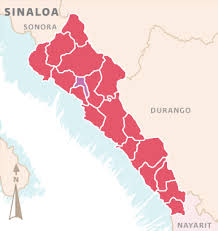
\includegraphics[width=0.36\textwidth]{Salvarado.jpg}
    \caption{\textit{Salvador Alvarado ubicado en el mapa de Sinaloa.}}
\end{wrapfigure}

En este caso, yo elegí la ciudad de Guamúchil, ya que es donde voy de vacaciones con mis familiares, por lo cual es un lugar que me gustaría investigar y conocer más acerca de su comportamiento climatológico ya que es una zona donde la agricultura tiene suma importancia para tanto para el municipio como la ciudad.

\section{Desarrollo}
	Las características principales de nuestra estación, son las siguientes: la ciudad se llama Guamúchil, ubicada en el municipio de Salvador Alvarado perteneciente al estado de Sinaloa. El número de la estación es 25037, las coordenadas espaciales son latitud 25.469444, longitud -108.091667 y altitud 44m, actualmente operando desde 1962, es decir hace unos 59 años. 
    
\begin{wrapfigure}{l}{0.35\textwidth} 

\includegraphics[width=0.35\textwidth]{Sinaloa.jpg}
\caption{\textit{Sinaloa ubicado a nivel nacional.}}
\end{wrapfigure}
    
    Cabe destacar que el Municipio cuenta con un excelente campo agrícola, ya que hace producir a más de 15 cultivos. Muchos de ellos básicos para la Agroindustria Regional y para los mercados de consumo nacional e internacional, tales como cártamo, trigo, soya, maíz, sorgo, hortalizas, garbanzo, hongos, frutas y pastos entre otros. La agricultura es una de las actividades principales. En el campo de la ganadería, las existencias de ganado en el Municipio se estiman a 65,565 cabezas, para lo cual estamos trabajando coordinadamente con SAGARPA tanto a nivel Estatal como Federal para allegarnos recursos suficientes, para los programas de apoyo a los productores. El comercio es el principal elemento para el desarrollo y sustento del municipio. El intercambio comercial, que muestra en su evolución económica, ha sido el motor que le ha dado vida a la gran concentración de población de la cabecera municipal.
    
    
    
\section{Gráficas estadísticas }

\subsection{Lluvia/mes, evaporación/mes }
	En la primera gráfica, podemos ver como es que se realizan las lluvias con respecto al tiempo que pasa, que en este caso esta medido en meses, ya que así tendremos una visión mas amplia de como es que a largo de un año en este lugar; los meses más abundantes de lluvias. En este caso las lluvias se realizan con mayor frecuencia en los meses de julio, agosto y septiembre. 
   
\begin{wrapfigure}{r}{0.4\textwidth} 
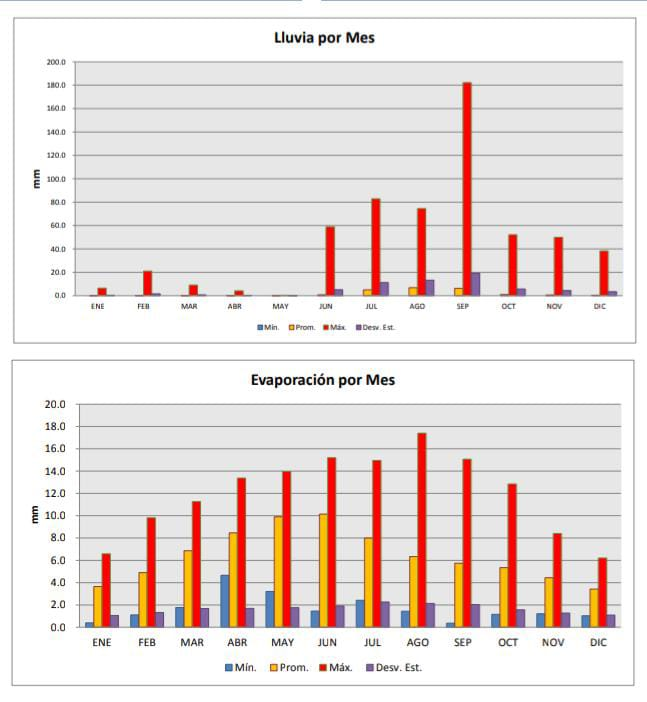
\includegraphics[width=0.4\textwidth]{Lluvias.jpeg}
\caption{\textit{Gráficas lluvia/mes, evaporación/mes.}}
\end{wrapfigure}

Ahora también si tomamos en cuenta la evaporación, podemos interpretar los datos como el aumento de la evaporación con respecto a los días más calurosos y con menos días de lluvias. Hay poca variación del clima, predominan fundamentalmente un clima tropical lluvioso en su parte oriental y clima seco estepario con lluvias en verano en el resto del municipio.
La temperatura media anual oscila entre los 24.2 y los 24.9 °C, con máximas que varían de 41 a 45 °C y mínimas de 3 a -3.5 °C. La precipitación media anual varía de 480 a 642 mm con un escurrimiento anual de aproximadamente 134 millones de m³.

\subsection{Promedio y máximo de precipitación}
Ahora en este caso, podemos ver que el promedio y máximo de lluvias, por década-mes, en la década de 2010 fue mas abundantes las lluvias con respecto a la década de 2000. 
La lluvia es vapor de agua que condensa en la atmósfera y cae al suelo a lo largo de un espacio considerable. 
El vapor condensado en superficie es lo que llamamos niebla. En la atmósfera hay siempre vapor de agua, pero este no condensa hasta que el aire se satura. 
La saturación depende de la temperatura.  A 100ºC se necesitan casi 0.6 gramos por litro de aire para la condensación, mientras que a 0ºC basta con casi nada, menos de una centésima de gramo para esa condensación. 

\begin{wrapfigure}{l}{0.35\textwidth} 
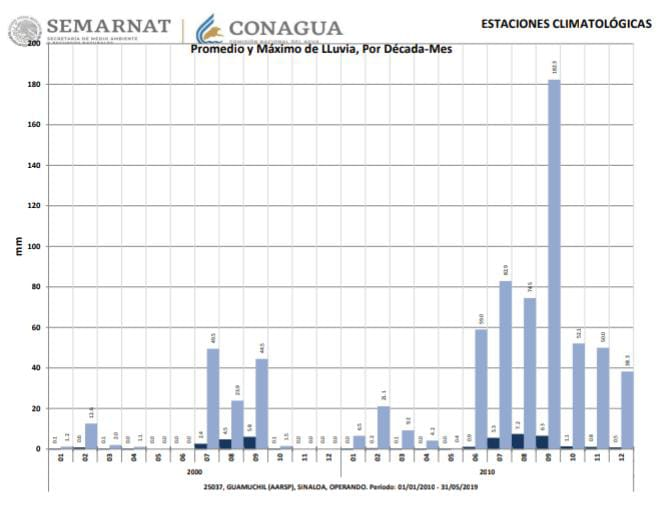
\includegraphics[width=0.35\textwidth]{Mlluvia.jpeg}
\caption{\textit{Promedio y máximo de lluvia, por década-mes.}}
\end{wrapfigure}

Por eso, en una mañana fría de invierno en un cuarto de baño con la calefacción sin poner, los espejos se llenan de gotitas de agua, mientras que esto no ocurre en verano, o con los radiadores encendidos en invierno.

\subsection{Promedio de lluvias diarias}
	La estación lluviosa, también conocida como temporada de lluvias o estación de los monzones, es la época del año en la cual se produce la mayor parte de la precipitación media anual de una región. Por lo general, tiene una duración de uno o varios meses. Si la temporada de lluvias se produce durante la estación cálida, o verano, la precipitación cae principalmente durante la tarde y las primeras horas de la noche. La temporada de lluvias suele ser el momento en que se puede observar una mejora de la calidad del aire y agua dulce, así como un crecimiento notable de la vegetación, culminando en consechas de los cultivos a finales de esta temporada. 
	
	\begin{wrapfigure}{r}{0.4\textwidth} 
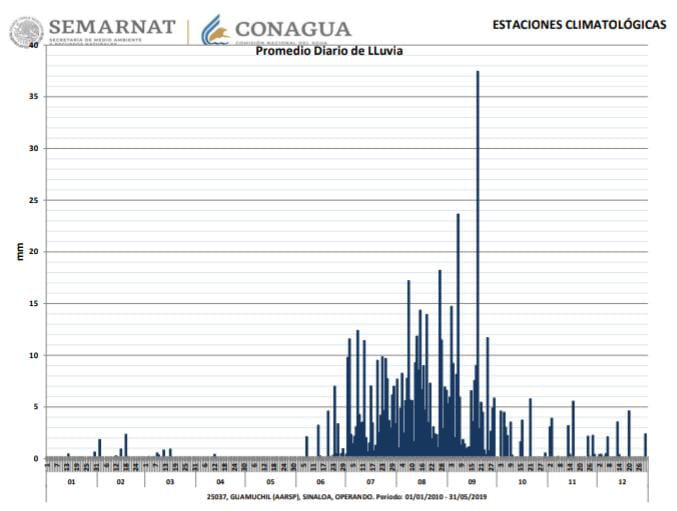
\includegraphics[width=0.4\textwidth]{Plluvia.jpeg}
\caption{\textit{Gráfica promedio diario de lluvias.}}
\end{wrapfigure}
	
	La precipitación puede causar inundaciones, y algunos animales se ven obligados a retirarse a terrenos más altos. Aumenta la erosión y disminuyen los nutrientes del suelo. La incidencia de malaria aumenta en las zonas donde la temporada de lluvias coincide con temperaturas elevadas. Los animales tienen estrategias de adaptación y de supervivencia para el régimen más húmedo. A menudo, la estación seca anterior conduce a la escasez de alimentos durante la temporada de lluvias, ya que los nuevos cultivos aún tienen que madurar.
	
\subsection{Registro diario de temperaturas máxima y mínima.}

		Interpretando los datos de nuestra gráfica podemos observar que son muy escasas las bajas temperaturas de la estación, ya que si acaso llega a alcanzar temperaturas bajas, llega a los 3 grados bajo cero, pero no es muy común el frio en esta región donde el promedio de temperaturas mínimas son alrededor de unos 17 grados, en el caso de las temperaturas altas, 
		
			\begin{wrapfigure}{r}{0.4\textwidth} 
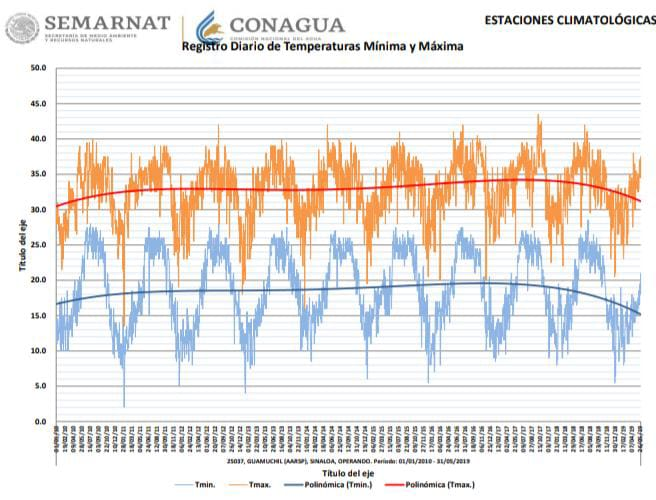
\includegraphics[width=0.4\textwidth]{Mtemperatura.jpeg}
\caption{\textit{Gráfica temperaturas máximas y mínimas.}}
\end{wrapfigure}
		
		podemos ver que si acaso unos 43 grados ha alcanzado esta estación,  y en periodos donde hay temperaturas altas, tenemos un promedio de temperatura de 38 grados, por lo mismo podemos concluir que cuenta con un clima perfecto para la agricultura como lo es en este caso, su fuerte.

\subsection{Registro diario de temperaturas máxima y mínima.}

		Ahora en el caso de los promedios, podemos observar un comportamiento similar al anterior, ya que podemos ver que existen ciertos factores que nos dicen como se está regulando la 
		
					\begin{wrapfigure}{r}{0.4\textwidth} 
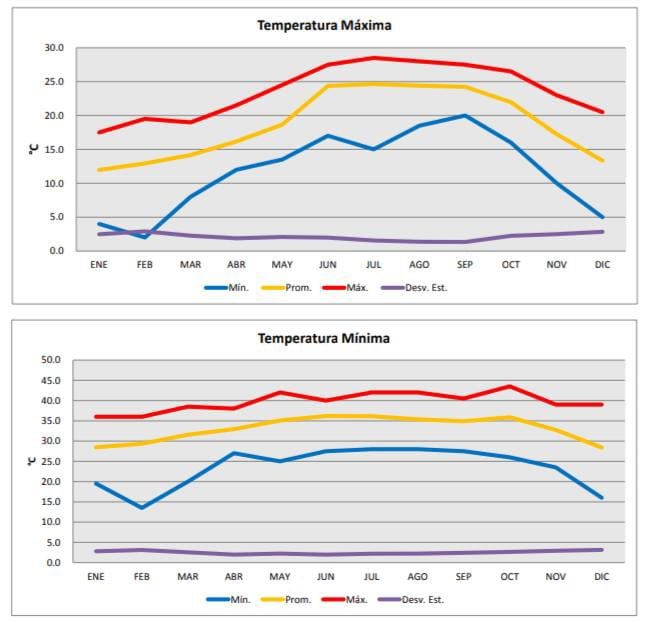
\includegraphics[width=0.4\textwidth]{Temperaturas.jpeg}
\caption{\textit{Gráfica promedios de temperaturas máximas y mínimas.}}
\end{wrapfigure}
		
		temperatura con respecto a nuestra variable principal que como lo es normalmente y como lo es en este caso la variable tiempo es la que nos influye en nuestro sistema de referencia y con respecto a el es que se están desarrollando los fenómenos estudiados. 
		


\section{Comentarios generales de la información}

A lo largo de la actividad, vimos e interpretamos lo datos de cada una de las gráficas presentes, ya que cada una de ellas representa los datos de un fenómeno en específico; los datos de un carácter específico de estudio en el campo, por ejemplo, las temperaturas, lluvias, precipitaciones, presión, entre otros comportamientos que se pueden dar en cualquier parte de esta zona. También cabe destacar que se hablo y se metió en contexto al lector , acerca de donde se ubica esta región y porque es importante estar en constaten estudio, ya que como es una de la zonas en México que tiene como sector primario la agricultura podemos ver que es de suma importancia para el país, es por eso que debemos estar siempre al pendiente de esta zona, ya que pueda que bajen las temperaturas de un día para otro y termine quemando toda la cosecha con el frio y así no ayudaría para nada a la agricultura del estado y mucho menos para el país.

\section{Bibliografía}

\textit{D. (s. f.). Información Estadística Climatológica. Gobierno de México. Recuperado 15 de enero de 2021, de https://smn.conagua.gob.mx/es/climatologia/informacion-climatologica/informacion-estadistica-climatologica}

\section{Apéndice}
\begin{enumerate}
\item \textbf{¿Qué te pareció?}\\
\textit{Me pareció muy bien la actividad, el combinar una actividad computacional con una de investigación de física, me gusto mucho ya que era algo que muy rara vez hacia antes y que ahora empiece el semestre con una como esta me llama mucho la atención..}

\item \textbf{¿Cómo estuvo el reto?}\\
\textit{Estuvo muy bien para empezar, ya que es cierto si nos hubieran dado las herramientas de trabajo antes, de seguro ni pudiéramos saber programar en LATEX, pero cuando dejan caer uno solo al agua y cuando uno se atora en el trabajo lo ayudan, creo que así se aprende de una mejor forma, y volviendo al reto creo que fue muy bueno para empezar e ir introduciéndose en el mundo de la programación enfocado a algo en concreto y en este software..}

\item \textbf{¿ ¿Qué se te dificultó más??} \\
\textit{El aprender a usar LATEX, ya que nunca antes lo habia intentado usar, pero lo bueno es que tengo compañeros que si saben y que me ayudaorn bastante.}

\item \textbf{¿Qué te aburrió?}\\
\textit{Nada en concreto, todo creo que fue de suma importancia y que en todo momento todo fue muy activo y dinámico.}

\item \textbf{¿Qué recomendarías para mejorar la primera Actividad?? }\\
\textit{Que también este el tiempo del sábado y del domingo para realizar la actividad, ya que me gustaría tener el fin de semana extra por si se necesitaban esos días extras.}

\item \textbf{¿Que grado de complejidad le asignarías a esta Actividad? (Bajo, Intermedio, Avanzado)} \\
\textit{Intermedio, ya que la única dificultad fue aprender a usar LATEX y en eso si me llevo mucho tiempo el aprender y saber usar correctamente los comandos.}

\end{enumerate}

\end{document}